\setcounter{section}{3}

\section{Скінченно-автоматні мови і праволінійні \allowbreak граматики}

\subsection{Скінченно-автоматні мови}

Ознайомившись з деякими результатами теорії скінчених автоматів, \allowbreak спробуємо з'я\-су\-ва\-ти, які мови (множини слів) є скінчено-автоматними.

\subsubsection{Базові мови}

\textbf{Твердження:} Скінчено автоматними є наступні множини:
\begin{enumerate}
	\item порожня словарна множина --- $\varnothing$;
	\item словарна множина, що складається з одного $\varepsilon$-слова --- $\{\varepsilon\}$;
	\item множина $\{a\}$, $a \in \Sigma$.
\end{enumerate}

\textbf{Доведення:} в кожному випадку нам доведеться конструктивно побудувати відповідний скінчений автомат:
\begin{enumerate}
	\item Довільний скінчений автомат з пустою множиною заключних станів (а мінімальний --- з пустою множиною станів) допускає $\varnothing$;
	\item Розглянемо автомат $M = \left\langle \{q_0\}, \Sigma, q_0, \delta, \{q_0\}\right\rangle$, у якому $\delta$ не визначено ні для яких $a \in \Sigma$. Тоді $L(M) = \{\varepsilon\}$.
	\item Розглянемо автомат $M = \left\langle \{q_0, q_1\}, \Sigma, q_0, \delta, \{q_1\}\right\rangle$, у якому функція $\delta$ визначена лише для пари $(q_0, a)$, а саме: $\delta(q_0, a) = \{q_1\}$. Тоді $L(M) = \{a\}$.
\end{enumerate}

\subsubsection{Операції над мовами}

\textbf{Твердження:} Якщо $M_1 = \left\langle Q_1, \Sigma, q_0^1, \delta_1, F_1 \right\rangle$ та $M_2 = \left\langle Q_2, \Sigma, q_0^2, \delta_2, F_2\right\rangle$, що визначають відповідно мови $L(M_1)$ та $L(M_2)$, то скінченно-автоматними мовами будуть:
\begin{enumerate}
	\item $L(M_1) \cup L(M_2) = \left\{w \mid q \in L(M_1) \text{ or } q \in L(M_2)\right\}$;
	\item $L(M_1) \cdot L(M_2) = \left\{w = xy \mid x \in L(M_1), y \in L(M_2) \right\}$;
	\item $L(M_1)^\star = \{\varepsilon\} \cup L(M_1) \cup L(M_1)^2 \cup L(M_1)^3 \cup \ldots$.
\end{enumerate}

\textbf{Доведення:} в кожному випадку нам доведеться конструктивно побудувати відповідний скінчений автомат:
\begin{enumerate}
	\item Побудуємо автомат $M = \left\langle Q, \Sigma, q_0, \delta, F \right\rangle$ такий, що $L(M) = L(M_1) \cup L(M_2)$:
	\begin{itemize}
		\item $Q = Q_1 \cup Q_2 \cup \{q_0\}$, де $q_0$ --- новий стан $(q_0 \notin Q_1 \cup Q_2)$;
		\item Функцію $\delta$ визначимо таким чином:
		\begin{equation}
			\delta(q, a) = \begin{cases}
				\delta_1(q, a), & q \in Q_1, \\
				\delta_2(q, a), & q \in Q_2, \\
				\delta_1(q_0^1, a) \cup \delta_2(q_0^2, a), & q = q_0. 
			\end{cases}
		\end{equation}
		\item Множина заключних станів:
		\begin{equation}
			F = \begin{cases}
				F_1 \cup F_2, & \text{if } \varepsilon \notin L_1 \cup L_2, \\
				F_1 \cup F_2 \cup \{q_0\}, & \text{otherwise}.
			\end{cases}		
		\end{equation}	
	\end{itemize}
	
	Побудований таким чином автомат взагалі кажучи недетермінований. \medskip

	Індукцією по $i$ показуємо, що $(q_0, w) \models^i (q,\varepsilon)$ тоді і тільки тоді, коли $(q_0^1,w) \models^i (q,\varepsilon), q \in F_1$ або $(q_0^2,w) \models^i (q,\varepsilon), q \in F_2$.
	\item Побудуємо автомат $M = \left\langle Q, \Sigma, q_0, \delta, F \right\rangle$ такий, що $L(M) = L(M_1) \cdot L(M_2)$:
	\begin{itemize}
		\item $Q = Q_1 \cup Q_2$;
		\item $q_0 = q_0^1$;
		\item Функцію $\delta$ визначимо таким чином:
		\begin{equation}
			\delta(q, a) = \begin{cases}
				\delta_1(q, a), & q \in Q_1 \setminus F_1, \\
				\delta_2(q, a), & q \in Q_2, \\
				\delta_1(q, a) \cup \delta_2(q_0^2,a), & q \in F_1.
			\end{cases}
		\end{equation}
		\item Множина заключних станів:
		\begin{equation}
			F = \begin{cases}
				F_2, & \text{if } \varepsilon \notin L_2, \\
				F_1 \cup F_2, & \text{otherwise}.
			\end{cases}
		\end{equation}
	\end{itemize}
	\item Побудуємо автомат $M = \left\langle Q, \Sigma, q_0, \delta, F \right\rangle$ такий, що $L(M) = L(M_1)^\star$:
	\begin{itemize}
		\item $Q = Q_1 \cup \{q_0\}$, де $q_0$ --- новий стан $(q_0 \notin Q_1)$;
		\item Функцію $\delta$ визначимо таким чином:
		\begin{equation}
			\delta (q, a) = \begin{cases}
				\delta_1(q, a), & q \in Q_1 \setminus F_1, \\
				\delta_1(q_0^1, a), & q = q_0, \\
				\delta_1(q, a) \cup \delta_1(q_0^1, a), & q \in F_1.
			\end{cases}
		\end{equation}
		\item Множина заключних станів $F = F_1 \cup \{q_0\}$.
	\end{itemize}
\end{enumerate}

\subsection{Скінченні автомати та праволінійні граматики}

\textit{Породжуюча граматика} $G$ --- це четвірка
\begin{equation}
	G = \left\langle N, \Sigma, P, S \right\rangle,
\end{equation}
де: 
\begin{itemize}
	\item $N$ --- скінченна множина --- допоміжний алфавіт (нетермінали);
	\item $\Sigma$ --- скінченна множина --- основний алфавіт (термінали);
	\item $P$ --- скінченна множина правил вигляду
	\begin{equation}
		\alpha \mapsto \beta, \quad \alpha \in \left(N \cup \Sigma\right)^\star \times N \times	\left(N \cup \Sigma\right)^\star, \quad \beta \in \left(N \cup \Sigma\right).
	\end{equation}
	\item $S$ --- виділений нетермінал (аксіома).
\end{itemize}

\subsubsection{Класифікація граматик Хомського}

В залежності від структури правил граматики діляться на чотири типи:
\begin{itemize}
	\item Тип 0: граматики загального вигляду, коли правила не мають обмежень, тобто
	\begin{equation}
		\alpha \mapsto \beta, \quad \alpha \in \left(N \cup \Sigma\right)^\star \times N \times	\left(N \cup \Sigma\right)^\star, \quad \beta \in \left(N \cup \Sigma\right).
	\end{equation}
	\item Тип 1: граматики, що не укорочуються, коли обмеження на правила мінімальні, а саме:
	\begin{equation}
		\alpha \mapsto \beta, \quad \alpha \in \left(N \cup \Sigma\right)^\star \times N \times	\left(N \cup \Sigma\right)^\star, \quad \beta \in \left(N \cup \Sigma\right), \quad |\alpha| \le |\beta|.
	\end{equation}
	\item Тип 2: контекстно-вільні граматики, коли правила в схемі $P$ мають вигляд:
	\begin{equation}
		A_i \mapsto \beta, \quad A_i \in N, \quad \beta \in \left(N \cup \Sigma\right)^\star.
	\end{equation}
	\item Тип 3: скінченно-автоматні граматики, коли правила в схемі $P$ мають вигляд:
	\begin{equation}
		A_i \mapsto w A_j, \quad A_i \mapsto w, \quad Ai \mapsto A_j w,
	\end{equation}
	де $A_i, A_j \in N$, $w \in \Sigma^\star$.
\end{itemize}

В класі скінченно-автоматних граматик виділимо так звані \textit{праволінійні граматики} --- це граматики, які в схемі Р мають правила вигляду:
\begin{equation}
    A_i \mapsto w A_j, \quad A_i \mapsto w,
\end{equation}
де $A_i, A_j \in N$, $w \in \Sigma^\star$. \medskip

Нескладно довести, що клас праволінійних граматик співпадає з класом граматик типу 3.

\subsubsection{Мова породжена граматикою}

Ланцюжок $w_1$ \textit{безпосередньо виводиться} з ланцюжка $w$ (позначається $w \Rightarrow w_1$), якщо $w = x \alpha y$, $w_1 = x \beta y$ та в схемі $P$ граматики $G$ є правило виду $\alpha \mapsto \beta$. Оскільки поняття ``безпосередньо виводиться'' розглядається на парах ланцюжків, то в подальшому символ $\Rightarrow$ буде трактуватися як бінарне вдіношення. \medskip

Ланцюжок $w_1$ \textit{виводиться} з ланцюжка $w$ (позначається $w \Rightarrow^\star w_1$), якщо існує скінчена послідовність виду $w \Rightarrow w_1' \Rightarrow w_2' \Rightarrow \ldots \Rightarrow w_n' \Rightarrow w_1$. Або кажуть, що бінарне відношення $\Rightarrow^\star$ --- це рефлексивно-транзитивне замикання бінарного відношення $\Rightarrow$. \medskip

\textit{Мова, яку породжує граматика} $G$ (позначається $L(G)$) --- це множина термінальних ланцюжків: 
\begin{equation}
    L(G) = \left\{ w \mid S \Rightarrow^\star w, w \in \Sigma^\star \right\}.
\end{equation}

\subsubsection{Праволінійна граматика \texorpdfstring{$\sim$}{~} скінченний автомат}

\textbf{Теорема.} \textit{Клас мов, що породжуються праволінійними граматиками, співпадає з класом мов, які розпізнаються скінченими автоматами.}

\textbf{Доведення.} Спочатку покажемо, що для довільної праволінійної граматики $G$ можна побудувати скінчений автомат $M$, такий що $L(M) = L(G)$. \medskip

Розглянемо правила праволінійної граматики. Вони бувають двох типів: $A_i \mapsto w A_j$, і $A_i \mapsto w$. \medskip

На основі правил граматики $G$ побудуємо схему $P_1$ нової граматики, яка буде еквівалентною початковій, а саме:
\begin{itemize}
	\item правила виду $A_i \mapsto a_1 a_2 \ldots a_p A_j$ замінимо послідовністю правил
	\begin{equation}
		\begin{aligned}
			A_i &\mapsto a_1 B_1, \\
			B_1 &\mapsto a_2 B_2, \\
			&\ldots \\
			B_{p - 1} &\mapsto a_p A_j.
		\end{aligned}
	\end{equation}
	\item правила виду $A_i \mapsto a_1 a_2 \ldots a_p$ замінимо послідовністю правил
	\begin{equation}
		\begin{aligned}
			A_i &\mapsto a_1 B_1, \\
			B_1 &\mapsto a_2 B_2, \\
			&\ldots \\
			B_{p - 1} &\mapsto a_p B_p, \\
			B_p &\mapsto \varepsilon.
		\end{aligned}
	\end{equation}
	де $B_1, B_2, \ldots$ --- це нові нетермінали граматики $G_1$.
\end{itemize}

Очевидно, що граматика $G_1$ ьуде еквівалентна граматиці $G$. \medskip

Далі, на основі граматики $G_1$ побудуємо скінчений автомат $M$, таким чином:
\begin{itemize}
	\item як імена станів автомата візьмемо нетермінали граматики $G_1$;
	\item початковий стан автомата позначається аксіомою $S$;
	\item функція $\delta$ визначається діаграмою переходів, яка будується на ос\-но\-ві правил вигляду $A_i \mapsto a_k A_j$:
	\begin{figure}[H]
		\centering
		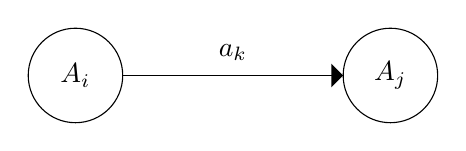
\begin{tikzpicture}[scale=0.2]
\tikzstyle{every node}+=[inner sep=0pt]
\draw [black] (0,0) circle (3);
\draw (0,0) node {$A_i$};
\draw [black] (20,0) circle (3);
\draw (20,0) node {$A_j$};
\draw [black] (3,0) -- (17,0);
\fill [black] (16.25,.75) -- (17,0) -- (16.25,-.75);
\draw (10,2) node [below] {$a_k$};
\end{tikzpicture}

	\end{figure}
	\item множина $F$ заключних станів скінченого автомата визначається так: $F = \{ A_i \mid A_i \mapsto \varepsilon \}$.
\end{itemize}

Індукцією по довжині вхідного слова покажемо, що якщо $S \Rightarrow^{n + 1} w$, то $(q_0, w) \models^n (q, \varepsilon)$:
\begin{itemize}
	\item База: $i = 0$: $S \Rightarrow \varepsilon$, тоді $(q_0, \varepsilon) \models^0 (q_0, \varepsilon)$.
	\item Перехід: нехай $|w| = i + 1$, тобто $w = a w_1$. Тоді $S \Rightarrow a A_p \Rightarrow^i a w_1$ та $(q_0, a w_1) \models (q_i, w_1) \models^{i - 1} (q, \varepsilon)$, де $q \in F$.
\end{itemize}

Доведення навпаки є очевидним.

\subsection{Контрольні запитання}

\begin{enumerate}
	\item Які три базові скінченно-автоматні мови ви знаєте? % emptyset, {eps}, {a}
	\item Доведіть, що мови з попереднього питання справді є скін\-чен\-но-ав\-то\-мат\-ни\-ми.
	\item Які три операції над скінченно-автоматними мовами ви знаєте? % об'єднання, конкатенація (а-ля декартів добуток), ітераці
	\item Доведіть, що результати операцій з попереднього питання справді є скін\-чен\-но-ав\-то\-мат\-ни\-ми.
	\item Що таке породжуюча граматика? % четвірка (нетермінали, термінали, правила виведення, аксіома)
	\item Які чотири типи граматик за Хомським ви знаєте? % загальні; ті, що не вкорочуються; контекстно-вільні; скінченно-автоматні
	\item Що таке праволінійна граматика? % скінченно-автоматна у якій нові нетермінали з'являються виключно праворуч
	\item Дайте визначення безпосереднього виведення, виведення, породженої граматикою мови.
	\item Доведіть, що скінченний автомат це майже праволінійна граматика.
\end{enumerate}
